\chapter{Revisões de Literatura}

Na primeira parte do trabalho, foi realizada uma revisão sistemática da literatura com o objetivo de identificar estudos que investigassem a relação entre jogos \textit{multiplayer}, habilidades sociais e TDAH, o que naquele momento fazia parte do foco do trabalho. No entanto, ao entender o escopo do estudo, foi decidido focar apenas nas habilidades sociais e nos jogos \textit{multiplayer}, o que tornou necessária a realização de uma segunda revisão.
%\todo{to da duvida se mantenho como ta, q ta bem explicadinho ou so resumo msm}
Como o resultado da segunda revisão foi mais relevante para o trabalho, a primeira revisão não será detalhada neste capítulo, mas os resultados obtidos serão apresentados de forma resumida. A segunda revisão sistemática, por sua vez, está descrita em detalhes, incluindo a estratégia de busca, critérios de inclusão e exclusão, etapas de triagem e análise dos artigos selecionados.
\section{Primeira Revisão}

A primeira revisão, dado o método utilizado, se classifica melhor como uma revisão de escopo e foi conduzida com o objetivo de identificar estudos que abordassem a interseção entre os temas \textit{multiplayer}, \textit{habilidades sociais} e \textit{transtorno de déficit de atenção/hiperatividade} (TDAH). Foram consultadas quatro bases de dados científicas: PubMed\footnote{https://pubmed.ncbi.nlm.nih.gov}, SpringerLink\footnote{https://link.springer.com/search}, ScienceDirect\footnote{https://www.sciencedirect.com} e ACM Digital Library\footnote{https://dl.acm.org/action/doSearch}.


\subsection{Estratégia de Busca}

As buscas foram realizadas utilizando combinações específicas de termos, como \texttt{"Multiplayer"}, \texttt{"Social skills"}, \texttt{"Attention deficit hyperactivity disorder"} e suas variações, conforme ilustrado na Tabela~\ref{tab:buscas}. A partir do cruzamento das palavras-chave e com o período de tempo dos últimos 10 anos, considerando que o dia de consulta foi 2 de fevereiro de 2025, foram identificados inicialmente \textbf{582} trabalhos. Após a exclusão de documentos classificados como anais em congressos, restaram \textbf{422} referências para análise detalhada.
\begin{table}[htbp]
\centering
\small
\setlength{\tabcolsep}{3pt}
\renewcommand{\arraystretch}{1.1}
\caption{Número de registros por combinação de termos nas bases de dados}
\label{tab:buscas}
\resizebox{\textwidth}{!}{%
\begin{tabular}{|l|c|c|c|c|c|c|c|c|}
\hline
\textbf{Termo de busca} & \multicolumn{2}{c|}{\textbf{PubMed}} & \multicolumn{2}{c|}{\textbf{SpringerLink}} & \multicolumn{2}{c|}{\textbf{ScienceDirect}} & \multicolumn{2}{c|}{\textbf{ACM}} \\
\cline{2-9}
 & All & 2015 & All & 2015 & All & 2015 & All & 2015 \\
\hline
Multiplayer & 626 & 444 & 13,581 & 9,075 & 6,457 & 3,604 & 18,269 & 9,188 \\
"Social skills" & 9,093 & 5,677 & 60,495 & 37,332 & 40,112 & 19,227 & 6,384 & 4,450 \\
"Social skill" & 772 & 406 & 59,302 & 36,661 & 40,112 & 19,227 & 668 & 466 \\
ADHD & 53,217 & 26,490 & 50,782 & 34,505 & 56,672 & 33,606 & 1,691,497 & 886,099 \\
Attention deficit hyperactivity disorder & 49,362 & 23,652 & 58,543 & 37,620 & 78,158 & 42,180 & 1,996 & 1,591 \\
"Attention deficit hyperactivity disorder" & 34,787 & 19,126 & 44,713 & 30,269 & 57,702 & 33,143 & 1,646 & 1,334 \\
\hline
Multiplayer AND "Social skills" & 4 & 4 & 985 & 847 & 259 & 203 & 575 & 422 \\
Multiplayer AND "Social skill" & 0 & 0 & 953 & 820 & 259 & 203 & 73 & 61 \\
Multiplayer AND ADHD & 5 & 5 & 429 & 387 & 137 & 117 & 5,880 & 3,107 \\
Multiplayer AND "Attention deficit hyperactivity disorder" & 4 & 4 & 321 & 294 & 125 & 103 & 63 & 56 \\
ADHD AND "Social skills" & 527 & 319 & 7,336 & 5,192 & 4,339 & 2,405 & 2,491 & 1,835 \\
ADHD AND "Social skill" & 0 & 0 & 7,245 & 5,140 & 4,339 & 2,405 & 285 & 205 \\
"Attention deficit hyperactivity disorder" AND "Social skills" & 352 & 214 & 6,182 & 4,329 & 4,261 & 2,275 & 124 & 111 \\
"Attention deficit hyperactivity disorder" AND "Social skill" & 30 & 19 & 6,119 & 4,286 & 4,261 & 2,275 & 20 & 19 \\
\hline
Multiplayer AND ADHD AND "Social skills" & 0 & 0 & 223 & 205 & 47 & 39 & 526 & 387 \\
Multiplayer AND ADHD AND "Social skill" & 0 & 0 & 219 & 203 & 47 & 39 & 70 & 59 \\
Multiplayer AND "Attention deficit hyperactivity disorder" AND "Social skills" & 0 & 0 & 185 & 172 & 43 & 33 & 46 & 41 \\
Multiplayer AND "Attention deficit hyperactivity disorder" AND "Social skill" & 0 & 0 & 181 & 170 & 43 & 33 & 13 & 13 \\
\hline
\end{tabular}
}
\end{table}
\subsection{Critérios de Inclusão e Exclusão}

Para garantir a relevância e a qualidade metodológica dos estudos incluídos, foram adotados os seguintes critérios:

\textbf{Critérios de inclusão:}
\begin{itemize}
    \item Estudos publicados em periódicos científicos revisados por pares;
    \item Investigações que abordem, de forma direta, pelo menos dois dos três eixos temáticos: jogos \textit{multiplayer}, habilidades sociais e TDAH.
\end{itemize}

\textbf{Critérios de exclusão:}
\begin{itemize}
    \item Documentos que não sejam artigos científicos (ex: livros, capítulos, anais de congresso);
    \item Artigos indisponíveis em texto completo;
    \item Estudos que não tratem dos temas propostos (jogos \textit{multiplayer}, habilidades sociais, TDAH);
    \item Artigos que não abordam nenhum dos três eixos temáticos como foco principal;
    \item Trabalhos com falhas metodológicas graves, como  presença de viés de confirmação evidente entre outros;
    \item Não estar publicado em revistas de Classificação A1, segundo a plataforma Sucupira da Capes (métrica válida durante o período da revisão realizada).
\end{itemize}

\subsubsection{Etapas de Triagem}

A triagem dos \textbf{422 registros} foi realizada unicamente pelo autor e em três etapas:

\begin{enumerate}
    \item \textbf{Filtragem por tipo de documento:} Excluíram-se \textbf{193 documentos} por não se tratarem de artigos científicos revisados por pares (eram livros, capítulos ou anais em congressos).

    \item \textbf{Leitura de títulos e resumos:} Dos \textbf{229 documentos} restantes, foram excluídos:
    \begin{itemize}
        \item \textbf{131 artigos} por não abordarem diretamente TDAH, jogos \textit{multiplayer} ou habilidades sociais como foco central;
        \item \textbf{31 artigos} por não envolverem habilidades sociais;
        \item \textbf{24 artigos} por não incluírem jogos \textit{multiplayer} no contexto estudado;
        \item \textbf{10 artigos} por não estarem disponíveis em texto completo;
        \item \textbf{2 artigos} por apresentarem falhas metodológicas graves;
        \item \textbf{11 artigos} por não estarem publicados em revistas de classificação A1.
    \end{itemize}

    \item \textbf{Seleção final:} Após aplicação de todos os critérios, \textbf{20 artigos} atenderam plenamente aos critérios de inclusão e foram selecionados para análise aprofundada.
\end{enumerate}

\subsection{Artigos selecionados}
A partir da leitura completa dos artigos, foi possível agrupá-los em 5 tipos de trabalhos apresentados, conforme Tabela \ref{tab:tiposdetrabalho}.
%Tabelas tipos de artigos
\begin{table}[H]
\centering
\caption{Referências por tipo de trabalho e foco do estudo}
\label{tab:tiposdetrabalho}
\resizebox{\textwidth}{!}{%
\begin{tabular}{|p{4.3cm}|p{4.2cm}|p{10cm}|}
\hline
\textbf{Referência} & \textbf{Tipo de Trabalho} & \textbf{Foco do Trabalho} \\
\hline
\cite{Bailey2021} & Revisão Literária & \RaggedRight Realidade virtual ou aumentada e comunicação em pessoas com Transtornos do Neurodesenvolvimento ou TNDs \\\hline
\cite{Goncalves2023} & Revisão Literária & \RaggedRight Definição e compreensão do termo "jogos sociais" \\ \hline
\cite{Vacca2023} & Revisão Literária & \RaggedRight Aplicações terapêuticas de jogos sérios em TNDs \\\hline
\cite{Derks2022} & Revisão Literária & \RaggedRight Efeitos de jogos sérios em crianças com TEA ou DI \\\hline
\cite{Prizant2016} & Revisão Literária & \RaggedRight Relação entre ansiedade social e uso da internet \\\hline
\cite{Hewett2020} & Jogo como Ferramenta & \RaggedRight Minecraft como ambiente didático (aula) \\\hline
\cite{Jagannath2020} & Jogo como Ferramenta & \RaggedRight Minecraft como ferramenta de resolução de problemas (extra-curricular) \\\hline
\cite{Ruiz2018} & Jogo como Ferramenta & \RaggedRight Efeitos de Pokémon GO em cognição e sociabilidade \\\hline
\cite{Daniau2016} & Jogo como Ferramenta & \RaggedRight TRPGs para desenvolvimento pessoal e social \\\hline
\cite{López2020} & Aplicação de Jogo Sério & \RaggedRight Reconhecimento de emoções e regulação emocional \\\hline
\cite{Mittmann2022} & Aplicação de Jogo Sério & \RaggedRight Incentivo a busca por saúde mental de adolescentes \\\hline
\cite{Gray2019} & Aplicação de Jogo Sério & \RaggedRight Treinamento de funções executivas em crianças com TEA \\\hline
\cite{Bul2016} & Aplicação de Jogo Sério & \RaggedRight Apoio ao tratamento de crianças com TDAH \\\hline
\cite{Martoncik2016} & Análise de Comunidade & \RaggedRight Redução da solidão e ansiedade social em MMORPGs \\\hline
\cite{Silva2015} & Análise de Comunidade & \RaggedRight Estratégia e resolução de problemas em mundos virtuais \\\hline
\cite{Czauderna2024} & Análise de Comunidade & \RaggedRight Competências socioemocionais em jogadores de Elden Ring \\\hline
\cite{Maloney2020} & Análise de Comunidade & \RaggedRight Comunicação não verbal em jogos de VR \\\hline
\cite{AlonsoDiaz2019} & Análise de Comunidade & \RaggedRight Desenvolvimento de competências por meio de videogames \\\hline
\cite{Feelings2023} & Análise de Comunidade & \RaggedRight Presença e suporte social em realidade virtual  \\\hline
\cite{Maitland2018} & Criação de Ferramenta & \RaggedRight Ferramenta para medir o potencial de interação social de \textit{Active Games} \\\hline
\hline
\end{tabular}
}
\end{table}


\subsubsection{Tipo 1: Revisões de Literatura}
% 1


% -----------------------------------------------------
\begin{table}[H]
\centering
\caption{ Revisões incluídas na análise}
\label{tab:revisoes}
\resizebox{1.1\textwidth}{!}{%
\begin{tabular}{|l|p{9cm}|l|c|c|}
\hline
\textbf{Referência} & \textbf{Foco} & \textbf{Meta-análise} & \textbf{Artigos} & \textbf{Período} \\
\hline
\cite{Bailey2021} & Jogos de realidade virtual ou aumentada aplicada em pessoas com deficiência de comunicação e transtornos do neurodesenvolvimento & Não & 69 & até 2020 \\\hline
\cite{Derks2022} & Aplicação de SG em crianças com TEA ou DI em experimentos clínicos randomizados & Sim & 11 & até 2020 \\\hline
\cite{Goncalves2023} & Jogos sociais & Não & 263 & 1990--2021 \\\hline
\cite{Prizant2016} & Ansiedade social na internet & Sim & 23 & 1990--2013 \\\hline
\cite{Vacca2023} & Aplicação de SG em distúrbios neurológicos & Não & 158 & 2010--2023 \\
\hline
\end{tabular}
}
\end{table}

Apesar de cada revisão ter um foco bem específico, todas tangenciam a área dos Jogos e algumas trazem informações realmente interessantes para o presente trabalho. O trabalho de \citeautor{Bailey2021} focou em analisar Jogos de realidade aumentada ou virtual e ao verificar que existem vários métodos e ferramentas para trabalhar com essa tecnologia ele conseguiu inferir que a viabilidade dessas ferramentas ainda é limitada, mas alguns artigos sugerem que VR/AR pode oferecer experiências de aprendizagem seguras e autênticas para pessoas com TEA, deficiência intelectual e distúrbios de comunicação.
% 2
%\marginnote{\footnotesize\textbf{Comentário:} \textcolor{red}{acho q tenho q escrever mais sobre o \cite{Bailey2021}, ficou meio pequeno a citação}}


A revisão de \citeautor{Derks2022} focou em verificar eficácia dos jogos sérios como ferramenta terapêutica, para desenvolver as habilidades sociais e cognitivas de crianças com deficiência intelectual (DI) e/ou transtorno do espectro autista (TEA), a qualidade dos artigos selecionados foi verificada com a ferramenta \textit{Cochrane Risk of Bias V2}, \cite{higgins2008cochrane}, que considera cinco domínios: aleatorização, desvios da intervenção, dados ausentes, medição dos resultados e seleção dos resultados relatados.

O tamanho do efeito foi considerado pequeno a moderado (g = 0,420), indicando que, em média, as crianças que utilizaram jogos sérios se saíram melhor do que aquelas que não os utilizaram. Esse valor de g corresponde ao \textbf{Hedges' g} \cite{hedges1985statistical}, uma medida estatística que quantifica a diferença padronizada entre dois grupos. Um valor de 0,420 sugere um efeito modesto, porém significativo (p = 0,009), reforçando a efetividade da intervenção.

Outro indicador importante foi o \textbf{NNT}  = 4,28, o que significa que, para cada quatro crianças que utilizam jogos sérios, uma apresenta melhora significativa atribuída a intervenção. A análise também mostrou moderada heterogeneidade entre os estudos (I² = 56,6\%), o que sugere que os resultados variavam razoavelmente entre os trabalhos incluídos. Mesmo após a exclusão de três estudos com alto impacto, os efeitos permaneceram estatisticamente significativos, embora ligeiramente reduzidos, e a heterogeneidade foi eliminada.
% 3

Já na revisão de \citeautor{Goncalves2023} foi notoriamente interessante, pois trouxe uma classificação de que a literatura necessitava sobre o que é um ``Jogo Social''. Seu trabalho trouxe um espectro de nomenclaturas baseadas em trabalhos anteriores, aos quais cada um tinha uma definição, o que o autor coloca num espectro de quão ``social'' um jogo pode ser.

A primeira entende social como qualquer forma de jogo não-solitária, ou seja, com a participação de mais de uma pessoa, mesmo que não haja interação complexa, basta jogar junto para ser considerado social. A segunda categoria foca na intenção do jogo, um jogo é social quando é projetado para estimular interação entre os jogadores, por meio de mecânicas como chat, trocas ou cooperação. Já a terceira definição considera as interações durante ou fora do jogo, distinguindo interações motivadas pelo design das espontâneas e incluindo também comunidades, fóruns e relações pré-existentes entre jogadores. A quarta classificação vê o aspecto social nos resultados gerados pelo jogo, como fortalecimento de laços, novas amizades ou sentimentos de conexão, inclusive com personagens artificiais. Por fim, há a visão de que o social é inerente ao próprio jogo, mesmo nos modos \textit{single-player}, pois todo jogo envolve elementos sociais, culturais e comunicativos.
% 4

O trabalho de \citeautor{Prizant2016} investigou a relação entre ansiedade social e o uso da internet e seus resultados indicaram que pessoas com altos níveis de ansiedade social tendem a se sentir mais confortáveis interagindo no ambiente virtual do que presencialmente, com uma correlação de r = 0{,}34. Segundo os autores, o meio digital, por permitir anonimato e reduzir sinais de julgamento social, funciona como um espaço seguro para indivíduos com esse perfil.

Outro ponto importante da análise foi a ausência de pistas não verbais na comunicação online. A pesquisa demonstrou que esse fator contribui para a preferência digital entre os ansiosos, evidenciada por uma correlação positiva (r = 0{,}27) entre a ansiedade social e o alívio causado pela ausência de elementos como expressão facial ou tom de voz, destacando o peso da comunicação não verbal no sentimento de ansiedade social. No entanto, não houve uma relação estatisticamente significativa entre ansiedade social e o tempo total gasto online (r = 0{,}07), indicando que o fator determinante não é a quantidade de uso, mas o tipo de uso.

A análise também mostrou que pessoas com ansiedade social têm maior propensão ao uso problemático da internet (PIU -- \textit{Problematic Internet Use}), com uma correlação de r = 0{,}20. Isso foi particularmente evidente no tempo dedicado a jogos online (r = 0{,}26), que pareceram atrair mais esse público do que outras formas de interação digital, como e-mails ou mensagens instantâneas. Por fim, observou-se que a idade é um moderador importante: a relação entre ansiedade social e uso da internet é mais forte em adultos do que em adolescentes ou jovens.
% 5

O último artigo de revisão bibliográfica, escrito por \cite{Vacca2023}, traz um apanhado geral sobre os jogos sérios ou \textit{serious games} (SGs) como terapias digitais aplicadas ao tratamento de Transtornos do Neurodesenvolvimento (TNDs), como TEA, TDAH, Síndrome de Down (SD) e Síndrome do X Frágil (FXS).

Na primeira parte do artigo ele estabelece uma classificação sobre os SGs : \textit{(i)} jogos preventivos (voltados à promoção da saúde), \textit{(ii)} jogos de avaliação (utilizados para rastrear sintomas e défices), e \textit{(iii)} jogos terapêuticos (focados na reabilitação e cuidado). Na segunda parte ele discorre sobre as tecnologias envolvidas  no desenvolvimento desses SGs como realidade aumentada e virtual (AR/VR), sensores corporais, dispositivos vestíveis e sistemas inteligentes de feedback. Essas tecnologias possibilitam o monitoramento remoto e adaptativo das atividades, promovendo maior engajamento e eficácia terapêutica.

Por fim, os estudos mostram resultados positivos em intervenções com SGs, especialmente para o desenvolvimento de habilidades cognitivas, motoras e socioemocionais em crianças com TNDs. Alguns exemplos incluem melhoras em memória de trabalho, atenção seletiva, reconhecimento de emoções e regulação comportamental.

Os autores concluem que, embora os jogos sérios (SGs) representem uma alternativa promissora como intervenção digital para pessoas com TNDs, o campo ainda está em estágio inicial de desenvolvimento clínico. Há poucos ensaios clínicos randomizados, limitados a alguns transtornos como TEA e TDAH, sendo necessário ampliar os estudos para outras condições, como a síndrome de Down (DS) e a síndrome do X frágil (FXS).

\subsubsection{Tipo 2: Jogo como Ferramenta}
Neste subgrupo, todos os trabalhos tiveram experimentação com usuários reais e utilizaram jogos de entretenimento como ferramenta didática ou para analisar os efeitos deles na saúde intelectual de seus jogadores.


\begin{table}[H]
\centering
\caption{Estudos experimentais com jogos multiplayer}
\label{tab:experimentos-educacionais}
\resizebox{\textwidth}{!}{%
\begin{tabular}{|l|l|l|c|c|}
\hline
\textbf{Referência} & \textbf{Tempo} & \textbf{Foco} & \textbf{Amostra} & \textbf{Idade} \\
\hline
\cite{Hewett2020} & 6 semanas & Minecraft como ferramenta didática & 13 & 18+ \\\hline
\cite{Jagannath2020} & 6 meses & Minecraft como oficina extracurricular & 30 & 8 a 14 \\\hline
\cite{Ruiz2018} & 8 semanas & Análise dos efeitos de jogar Pokémon GO  & 190 & 12 a 15 \\\hline
\cite{Daniau2016} & \textasciitilde250h & Análise dos efeitos de jogar TRPG & \textasciitilde20 & 20 a 65 \\
\hline
\end{tabular}
}
\end{table}

Tanto o trabalho de \citeautor{Hewett2020} quanto de  \citeautor{Jagannath2020} utilizaram o jogo Minecraft\footnote{https://www.minecraft.net/pt-br} como ambiente de estudo, e apesar de suas abordagens serem diferentes ambos trouxeram resultados e conclusões semelhantes.
Em \citeautor{Hewett2020}, o autor observou 13 estudantes do ensino médio da região sul do Texas em seis projetos com Minecraft, investigando como desenvolviam as definidas ``habilidades do século XXI'' ou Quatro Cs: criatividade, pensamento crítico, comunicação e colaboração.

A coleta de dados foi feita por meio de entrevistas, observações diretas durante as construções no jogo, fotos e capturas de tela, o pesquisador também  participou dos projetos como observador para se inserir no ambiente virtual e acompanhar o processo dos alunos. A análise seguiu uma abordagem interpretativa e qualitativa para interpretar as atitudes e respostas dos alunos.

Já o trabalho de \citeautor{Jagannath2020} teve um enfoque maior na observação através do \textbf{Survival Lab}, uma atividade extracurricular desenvolvida no jogo Minecraft, voltada para jovens de 8 a 14 anos. O programa foi constituído de sessões de 90 minutos, duas vezes por semana, durante seis meses. Os participantes enfrentaram desafios em equipe e participaram de narrativas diversas, como aventuras no deserto ou no espaço.

A coleta de dados foi feita com pesquisadores observando em modo espectador e utilizando gravações de áudio, vídeo, capturas de tela, chats e anotações de campo. A equipe incluía quatro moderadores universitários e um voluntário do ensino médio. As atividades incluíam  discussões de abertura e encerramento e desafios cooperativos. A análise dos dados foi conduzida por meio de dados qualitativos, buscando compreender como os participantes interagiam, desenvolviam habilidades sociais e se engajavam nas dinâmicas no jogo.

Em suma, os dois trabalhos ressaltam o potencial do Minecraft como uma ferramenta eficaz no desenvolvimento de habilidades socioemocionais e cognitivas como resolução de problemas, raciocínio lógico, tomada de decisões entre outros. As evidências relatadas, apesar de apenas qualitativas, indicam que ao interagir em ambientes virtuais colaborativos, os participantes demonstram autonomia, criatividade e cooperação. Tanto no \textit{Survival Lab} de \cite{Jagannath2020} quanto no estudo de \cite{Hewett2020}, os jovens se organizaram espontaneamente e atuaram em equipe, além disso, ambos os autores reforçam que o aprendizado mediado pelo Minecraft gera ambientes ricos para a experiência social dos participantes.

% 3

Já em \citeautor{Ruiz2018} é apresentada uma análise quantitativa dos efeitos de Pokémon GO\footnote{https://pokemongo.com/pt-BR}, um jogo \textit{mobile} de realidade aumentada, sobre o desempenho cognitivo e a inteligência emocional de adolescentes. Os instrumentos psicométricos utilizados foram testes \textit{ad hoc} de memória, atenção seletiva e concentração (teste d2), cálculo matemático e compreensão linguística. A IE foi medida por meio do \textit{Trait and Emotional Intelligence Questionnaire Short Form} -- TEIQue-SF \cite{petrides2009teique}, que avalia dimensões como bem-estar, autocontrole, emocionalidade e sociabilidade.

Os participantes foram avaliados antes e após um período de oito semanas de uso contínuo do jogo. Durante esse período, os adolescentes jogaram \textit{Pokémon GO} livremente, e os dados de engajamento (nível no jogo, distância percorrida e tempo de jogo) foram coletados diretamente do aplicativo. Para a análise estatística, foram empregados testes \textit{t} de Student, ANCOVA para medidas repetidas e correlações de Spearman.

Ao final do experimento os participantes apresentaram melhorias significativas na atenção seletiva (13,26\% a mais que o grupo controle) e na concentração (aumento de 19,4\%), além de um crescimento na sociabilidade (9,87\% superior). No entanto, não foram observadas mudanças significativas em memória, raciocínio linguístico, cálculo matemático, bem-estar ou autocontrole, os jovens relataram estar mais motivados, felizes e dispostos a sair de casa devido ao jogo sendo que os meninos demonstrando maior engajamento e benefício percebido.
%4

O artigo de \citeautor{Daniau2016} foge um pouco do que se vem em mente quando é pensado em jogos \textit{multiplayer} por não se tratar de um jogo digital mas TRPGs, também conhecidos como RPGs de mesa podem nos trazer informações interessantes tanto do efeito de jogos multiplayer nos jogadores, quanto na forma de medir seus impactos.

A metodologia utilizada nesse artigo inclui longas sessões de jogo seguidas por relatórios colaborativos, em que aspectos emocionais, sociais e cognitivos da experiência eram analisados. O jogo era centrado em personagens com histórias complexas, ambientadas em mundos ficcionais inspirados em H.P. Lovecraft\footnote{Howard Phillips Lovecraft foi um escritor americano dos gêneros de weird fiction, ficção científica, fantasia e terror.}, favorecendo a imersão e a construção de significados compartilhados.

A pesquisa identificou quatro níveis de envolvimento do jogador: personagem (aprendizagem temática e cultural), jogador (habilidades básicas), pessoa (competências socioemocionais) e ser humano (aprendizagem transformadora). Esses níveis foram associados aos quatro pilares da educação propostos pela UNESCO: aprender a conhecer, fazer, ser e conviver. Os dados revelaram que a experiência com TRPGs favorece o desenvolvimento de habilidades como resolução de problemas, empatia, pensamento crítico, colaboração e criatividade.

Por fim, o autor argumenta que as propriedades únicas dos TRPGs — como a simulação de dilemas, a interação social estruturada e a narrativa coletiva — tornam essa prática especialmente eficaz em contextos educacionais, terapêuticos e de formação de equipes. Ao conectar os elementos do jogo com experiências reais dos participantes, esses jogos favorecem processos de conscientização.

\subsubsection{Tipo 3: Aplicação de Jogo Sério}
Os artigos mencionados a seguir tratam de trabalhos de desenvolvimento e experimentação de jogos sérios em crianças de até 13 anos de idade.


\begin{table}[H]
\centering
\caption{Estudos com aplicação de jogos sérios}
\label{tab:seriousgames}
\resizebox{\textwidth}{!}{%
\begin{tabular}{|l|c|p{6.5cm}|c|c|}
\hline
\textbf{Referência} & \textbf{Tempo} & \textbf{Foco} & \textbf{Amostra} & \textbf{Faixa etária} \\
\hline
\cite{López2020} & ~4,75h & Desenvolvido para percepção e regulação emocional & 38 & 9 a 11 \\\hline
\cite{Mittmann2022} & ~5h & Redução do estigma relacionado a saúde mental & 91 & 10 a 13 \\\hline
\cite{Gray2019} & 5 semanas & Treinar habilidades de função executiva & 31 & 11 a 12 \\\hline
\cite{Bul2016} & 20 semanas & Melhora na gestão do tempo e habilidades sociais & 170 & 8 a 12 \\
\hline
\end{tabular}
}
\end{table}

% 1
O trabalho de \citeautor{López2020} trata-se do \textbf{EmoFindAR}, um jogo sério de realidade aumentada para dispositivos móveis e \textit{multiplayer} construído para crianças de 9 a 11 anos com o objetivo de ajudá-las a reconhecer, compreender e regular emoções básicas (alegria, tristeza, raiva etc.) além de promover habilidades de comunicação e colaboração. O jogo apresenta modos competitivo e colaborativo, nos quais os jogadores devem interagir com personagens virtuais espalhados pelo ambiente físico, e lançar objetos que modificam seu estado emocional até que possam ser "capturados", uma mecânica extremamente semelhante ao jogo \textbf{Pokemon GO}.

O estudo experimental foi conduzido com 38 crianças do 5º ano, onde cada dupla jogou nos dois modos (competitivo e colaborativo). A ferramenta foi desenvolvida utilizando a Engine Unity\footnote{https://unity.com/pt}, além de\textit{Photon Unity Networking}\footnote{https://www.photonengine.com/PUN} e o SDK Plaecnote\footnote{https://developer.android.com/tools/releases/platform-tools?hl=pt-br} para posicionamento 3D, a coleta de dados envolveu questionários e observações de comportamentos. Os resultados mostram que no modo competitivo, houve uma maior motivação individual entre os participantes, que se empenharam para capturar o maior número de personagens e vencer a partida estimulando respostas mais rápidas e maior atividade física, enquanto no modo cooperativo os jogadores precisaram agir em conjunto e coordenar suas ações em tempo real, já que a captura dos personagens exigia a atuação sincronizada dos dois participantes, o que reforçou o desenvolvimento de habilidades sociais e emocionais entre os alunos.

% 2
O jogo desenvolvido por \citeautor{Mittmann2022}, \textbf{Lina} trata sobre um assunto pouco trabalhado na área de jogos sérios, que é justamente saúde mental. Em Lina uma turma inteira, incluindo professor, entram em uma narrativa e interativa, utilizando um aplicativo movel e realidade aumentada, a turma investiga o desaparecimento de uma colega fictícia chamada Lina, que lidava com uma situação familiar difícil, O enredo e os desafios do jogo incentivam a colaboração, comunicação, e reflexão coletiva, abordando temas de exclusão social, empatia e diferenças individuais.

O questionário \textbf{GUESS-18}\cite{Keebler2020}, aplicado para avaliar o jogo, apresentou boa confiabilidade interna ($\alpha = 0,83$), com pontuação total de usabilidade de 33,64. As dimensões mais bem avaliadas foram diversão (média = 4,42) e conectividade social (média = 4,37), enquanto liberdade criativa, envolvimento, gratificação pessoal e usabilidade tiveram escores mais baixos, explicados por limitações estruturais do jogo e problemas técnicos, dado que ainda era um protótipo.

Nos grupos focais, discussões semiestruturadas conduzidas com pequenos grupos de 3 a 4 adolescentes cada, os adolescentes relataram uma experiência amplamente positiva, destacando a diversão, a colaboração entre colegas e o fortalecimento do sentimento de pertencimento. A narrativa foi compreendida, com ênfase nas temáticas de \textit{bullying} e exclusão social, e a participação de professores e o uso de dramatização foram considerados elementos que aumentaram o engajamento e a imersão na experiência.
% 3

O \textit{BrainQuest}, desenvolvido por \cite{Gray2019}, é uma aplicação \textit{mobile} voltada para crianças de 10 a 13 anos, com o objetivo de estimular o desenvolvimento de funções executivas, como atenção seletiva, controle inibitório e flexibilidade cognitiva. O jogo propõe desafios físicos, sociais e estratégicos realizados em espaços ao ar livre, sendo sua estrutura inspirada no teste \textbf{Modified Six Elements}\footnote{\textbf{Modified Six Elements}:  questionário utilizada para avaliar funções executivas. \cite{Venning2015}.}, a fim de proporcionar uma experiência lúdica e motivadora que favoreça o aprimoramento de habilidades cognitivas essenciais para essa fase do desenvolvimento infantil.

Uma característica central do \textit{BrainQuest} é a utilização da tecnologia \textbf{NFC} (\textit{Near Field Communication}), que permite a integração entre o ambiente físico e o virtual por meio de objetos do jogo, como vacas e ovelhas equipados com etiquetas NFC. Ao interagir fisicamente com esses elementos, as crianças vivenciam uma experiência de realidade mista, na qual a pontuação é calculada com base no cumprimento correto das tarefas e na alternância entre diferentes tipos de atividades, incentivando a variedade de estratégias e o raciocínio flexível.

O desenvolvimento do \textit{BrainQuest} foi fundamentado na \textit{Self-Determination Theory} (SDT), que enfatiza três pilares essenciais para promover o engajamento intrínseco: competência, autonomia e relacionamento social \cite{Deci2000}. Ao contrário de abordagens tradicionais de \textit{gamification}, o jogo foi projetado para oferecer desafios que envolvem não apenas capacidades cognitivas, mas também aspectos emocionais e sociais, promovendo o desenvolvimento das chamadas \textit{Hot Executive Functions} — aquelas relacionadas à regulação emocional, ao controle inibitório e à flexibilidade cognitiva em contextos que exigem motivação e interação social \cite{Zelazo2012}.

A aplicação foi testada em ambiente escolar, ao longo de cinco semanas, no contexto das aulas de educação física. Os resultados preliminares indicaram alto nível de aceitação e envolvimento por parte das crianças participantes, o que reforça o potencial do \textit{BrainQuest} para fomentar o desenvolvimento de habilidades executivas nessa faixa etária \cite{Gray2019}.
% 4

Por fim, o último estudo avaliou os efeitos do jogo sério \textit{Plan-It Commander} como intervenção complementar ao tratamento usual de crianças diagnosticadas com Transtorno de Déficit de Atenção e Hiperatividade. O público-alvo foi composto por crianças com idades entre 8 e 12 anos, majoritariamente do sexo masculino (80,6\%) \cite{Bul2016}. O objetivo principal do jogo foi promover melhorias em habilidades essenciais para a vida cotidiana dessas crianças, como gestão do tempo, organização e comportamento cooperativo, utilizando uma abordagem interativa baseada em princípios de aprendizado comportamental e \textit{game-based learning} \cite{Bul2016}.

A experimentação foi feita por um ensaio clínico randomizado, com duração total de 20 semanas. Os participantes foram divididos em dois grupos, onde, um utilizou o jogo nas primeiras 10 semanas, enquanto o outro o utilizou apenas nas 10 semanas finais, ambos mantendo o tratamento usual (medicação e/ou psicoterapia) durante todo o período.
A eficácia da intervenção foi avaliada  utilizando de questionários aplicados a pais, professores e às próprias crianças, contemplando aspectos como habilidades organizacionais, gestão do tempo, memória de trabalho, habilidades sociais e autoeficácia, e a análise foi feita utilizando métodos estatísticos da literatura como ANCOVAs entre outros. \cite{Bul2016}.

Os resultados apontaram que as crianças que utilizaram o \textit{Plan-It Commander} apresentaram melhorias estatisticamente significativas na gestão do tempo (p = 0{,}004), responsabilidade social (p = 0{,}04) e memória de trabalho (p = 0{,}02), com efeitos pequenos a moderados \cite{Bul2016}. Essas melhorias foram observadas tanto em casa quanto na escola, indicando que as habilidades desenvolvidas no ambiente virtual foram transferidas para contextos da vida real. Além disso, pais e crianças relataram altos níveis de satisfação com a intervenção (notas médias entre 6,9 e 7,3) \cite{Bul2016}.

\subsubsection{Tipo 4: Análise de Comunidade}

Nesses artigos, todos os autores se propõem a analisar os efeitos que comunidades de jogos \textit{online multiplayer} têm na vida dos participantes dessas comunidades, desde a redução do sentimento de solidão desses jogadores até o desenvolvimento de habilidades sociais e emocionais.
% 1


\begin{table}[H]
\centering
\caption{Estudos sobre comunidades em jogos digitais}
\label{tab:comunidades}
\resizebox{\textwidth}{!}{%
\begin{tabular}{|p{3.8cm}|c|p{6cm}|c|c|}
\hline
\textbf{Referência} & \textbf{Tempo} & \textbf{Foco} & \textbf{Amostra} & \textbf{Faixa etária} \\\hline
\cite{Martoncik2016} & N/A & MMORPGs como forma de intervenção contra a solidão & 161 & 13 a 50 \\\hline
\cite{Silva2015} & 250h & Compreensão do potencial dos MMORPGs para organizações & 2 & N/A \\\hline
\cite{Czauderna2024} & N/A & Competências socioemocionais em jogadores de Elden Ring no Reddit & 2.363\textsuperscript{*} & N/A \\\hline
\cite{Maloney2020} & 82h & Comunicação não verbal em ambientes de VR & 30 & 18 a 65 \\\hline
\cite{AlonsoDiaz2019} & N/A & Desenvolvimento de competências por meio de videogames & 404 & 18 a 65 \\\hline
\cite{Feelings2023} & N/A & Presença e suporte social em realidade virtual & 1231 & 14 a 74 \\\hline

\end{tabular}
}
\begin{flushleft}
\footnotesize\textsuperscript{*} Representa a contagem de comentários analisados, não indivíduos.
\end{flushleft}
\end{table}

No experimento de \citeautor{Martoncik2016}, 161 jogadores de \textit{World of Warcraft} contatados por fóruns online responderam a questionários padronizados que avaliavam solidão (por meio da Escala de Solidão da UCLA \cite{russell1996ucla}) e ansiedade social (por meio do Inventário de Fobia Social – SPIN\cite{connor2000spin}).
Esses questionários foram adaptados para que os jogadores respondessem separadamente considerando o mundo real e o mundo online.
Os dados demográficos e comportamentais incluíram afiliação a guildas, jogo com amigos, tempo médio semanal e total de jogo, além da frequência de uso de programas de comunicação, como TeamSpeak\footnote{Ferramenta de comunicação online comumente relacionada a jogos: https://www.teamspeak.com/en}.

Após análises estatísticas, os resultados indicaram diferenças significativas entre os valores de solidão e ansiedade social no mundo real e no mundo online, com menores níveis percebidos no ambiente virtual.
Os autores afirmam que tanto a solidão quanto a ansiedade social foram mais baixas no mundo online, com efeitos pequenos para solidão e grandes para ansiedade social.
Foi comprovado também que jogar com pessoas conhecidas e ser membro de guildas se associaram a níveis mais baixos de solidão, especialmente no mundo online.
A comunicação frequente com outros jogadores também reduziu tanto a solidão quanto a ansiedade social nesse contexto.
No entanto, o tempo total de jogo não apresentou efeito significativo sobre essas variáveis em nenhum dos ambientes.

Por fim, o estudo revela que, no geral, jogadores de MMORPG, como \textit{World of Warcraft}, tendem a experienciar menor solidão e ansiedade social no ambiente online em comparação ao mundo real. No entanto, o tempo total de jogo não mostrou relação direta com solidão ou ansiedade, indicando que a qualidade das interações sociais é mais relevante do que a quantidade de tempo gasto no jogo. Os autores propõem que MMORPGs podem servir como uma forma de intervenção contra a solidão por promoverem habilidades sociais e oportunidades de interação; todavia, alertam que o uso desses jogos como substituto do mundo real requer atenção e sugerem alternativas que promovam conexões sociais fora do ambiente virtual.

% 2
No trabalho de \citeautor{Silva2015}, os pesquisadores utilizaram o método de \textit{autoetnografia}, uma abordagem qualitativa em que o próprio pesquisador se insere como participante ativo do fenômeno estudado.
Durante três meses, eles jogaram \textit{World of Warcraft} a partir do nível inicial, sem experiência prévia com jogos do tipo MMORPG, registrando aproximadamente 500 páginas de descrições densas da experiência, que incluíam interações com o ambiente do jogo, outros jogadores e fontes externas, como fóruns e sites especializados.
A análise dos dados foi conduzida de forma que cada pesquisador identificou passagens relacionadas ao pensamento estratégico, categorizou temas emergentes e, posteriormente, discutiu os achados em conjunto.

Os resultados da pesquisa foram organizados em temas, onde o primeiro mostra que jogadores iniciantes interpretam o jogo com base em experiências do mundo real, mas, com o tempo, passam a basear suas decisões em experiências adquiridas no próprio jogo.
O segundo tema evidencia que o pensamento estratégico em \textit{WoW} envolve planejamento de ações, economia de recursos e cooperação com outros jogadores, sendo essencial para o sucesso em tarefas complexas como masmorras e \textit{raides}\footnote{Termo utilizado para classificar eventos ou missões cooperativas de grande escala, geralmente projetadas para grupos numerosos de jogadores, com o objetivo de derrotar chefes poderosos (\textit{bosses}), enfrentar desafios complexos e conquistar recompensas valiosas}.
O terceiro tema destaca que mesmo interpretações incompletas das tarefas não impedem os jogadores de agir, sendo o aprendizado mediado por recursos externos e pela experiência progressiva no jogo.
Por fim, o quarto tema revela que diante de situações novas ou sob pressão social, o jogador frequentemente age por imitação e só posteriormente compreende o sentido estratégico de suas ações — fenômeno interpretado como \textit{telescoping reverso}\footnote{Conceito proposto no artigo para descrever um tipo específico de raciocínio estratégico que acontece depois da ação.}.

Os autores concluem que o pensamento estratégico em ambientes de jogos MMORPGs, como \textit{World of Warcraft}, é construído socialmente e depende fortemente da experiência acumulada e da interação com fontes externas de conhecimento,além de que, em situações de incerteza, os jogadores iniciantes recorrem a interpretações parciais baseadas em experiências prévias e à imitação de outros jogadores, comportamento que diminui à medida que ganham familiaridade com o ambiente do jogo.
Nesse contexto, destaca-se o conceito de \textit{telescoping} concebido no trabalho, que descreve a capacidade de planejar e articular sequências de ações visando objetivos de curto e longo prazo, competência essencial no pensamento estratégico. Além disso, a coleta e utilização de informações provenientes de fóruns, guias e interações sociais evidenciam a natureza coletiva da formulação de estratégias.
Com isso, o artigo sugere que MMORPGs podem ser utilizados como laboratórios sociais para o desenvolvimento de habilidades estratégicas aplicáveis ao planejamento de sistemas de informação (SI), já que assim como em SI, os jogadores precisam analisar problemas complexos, tomar decisões sob incerteza, planejar ações com visão de curto e longo prazo e colaborar com outros.

% 3

O  estudo de \citeautor{Czauderna2024} investigou como jogadores demonstram competências socioemocionais em ambientes informais de aprendizagem, especificamente na página do \textit{Reddit}\footnote{https://www.reddit.com} dedicado ao jogo Elden Ring.
Utilizando uma análise temática qualitativa com base no modelo teórico da \textbf{CASEL}\footnote{https://casel.org} (\textit{Collaborative for Academic, Social, and Emotional Learning}), os autores analisaram um tópico popular da comunidade r/Eldenring com mais de 2 mil comentários e quase um milhão de visualizações.
As postagens foram codificadas com categorias como “filosofar”, “encorajar”, “estrategizar” e “empatizar”, sendo posteriormente agrupadas nas cinco competências da CASEL: autoconhecimento, autocontrole, consciência social, habilidades de relacionamento e tomada de decisão responsável, essa classificação permitiu identificar padrões de interação e comportamentos associados às competências socioemocionais.

Os resultados demonstraram que os jogadores apresentaram autoconhecimento ao refletir sobre suas emoções e frustrações com o jogo, e autocontrole ao compartilhar estratégias para lidar com o estresse, como fazer pausas ou mudar de abordagem.
A consciência social foi visível nas demonstrações de empatia entre novatos e veteranos, e nas mensagens de incentivo e compreensão mútua.
Já as habilidades de relacionamento foram evidenciadas em atitudes colaborativas, como responder dúvidas, dar conselhos e valorizar diferentes estilos de jogo.
Por fim, a tomada de decisão responsável foi observada nas estratégias discutidas para lidar com os desafios do jogo, além de reflexões sobre o aprendizado e crescimento pessoal promovidos pela experiência.

Como conclusão, o artigo sustenta que jogos desafiadores como Elden Ring, aliados aos espaços de discussão online, como o Reddit, podem ser poderosas ferramentas de aprendizagem socioemocional.
Mesmo em ambientes digitais anônimos, os jogadores demonstram competências relevantes para a vida pessoal e social, como resiliência, empatia, cooperação e reflexão ética.

% 4
Já no trabalho de \citeautor{Maloney2020}, foi investigado como a comunicação não verbal ocorre em ambientes de realidade virtual social, com foco nas interações entre usuários em plataformas como AltspaceVR\footnote{https://www.meta.com/pt-br/experiences/altspacevr/2133027990157329} e VRChat\footnote{https://hello.vrchat.com}.
O objetivo era entender que tipos de comportamentos não verbais surgem naturalmente nesses ambientes e como esses gestos afetam as interações sociais.
Antes de explicar os resultados, é preciso entender o contexto em que os jogadores estão envolvidos.
Jogos de realidade virtual sociais (social VR) são ambientes virtuais tridimensionais onde múltiplos usuários interagem em tempo real por meio de avatares imersivos, utilizando dispositivos como headsets de realidade virtual.
E diferente de alguns jogos de realidade virtual onde existe uma fase ou um objetivo específico, nos \textbf{social VR} a interação social é o objetivo do jogo, e não um efeito colateral.

Dentro desse contexto, foram realizados dois estudos: o primeiro consistiu em observações não intrusivas em eventos públicos na plataforma AltspaceVR, totalizando 82 horas de registros.
No segundo estudo, entrevistaram 30 usuários de diferentes perfis para entender suas percepções e experiências com a comunicação não verbal em social VR.

Após a análise foi comprovado que comportamentos não verbais como gestos, olhares, aplausos, proximidade e expressões faciais são usados de maneira espontânea e significativa.
Os participantes relataram que esses gestos tornam a comunicação mais natural, imersiva e confortável, especialmente para iniciantes, pessoas introvertidas ou membros de grupos marginalizados, como mulheres, pessoas trans e não falantes nativos de inglês.

Por fim, os autores afirmam que a comunicação não verbal em social VR oferece alternativas ao uso da voz, promove a sensação de presença e pertencimento e pode proteger a privacidade dos usuários.
O estudo destaca a importância de projetar plataformas mais inclusivas, com suporte aprimorado a comportamentos não verbais.


% 5
No trabalho de \citeautor{AlonsoDiaz2019}, foi investigado não apenas uma comunidade de jogadores específica, mas várias ao mesmo tempo e compararam suas possíveis contribuições para o desenvolvimento de competências-chave em adultos. O estudo teve como objetivo identificar se diferentes gêneros de jogos favorecem o aprimoramento de habilidades técnicas (\textit{hard skills}) e socioemocionais (\textit{soft skills}) entre jogadores adultos.

A pesquisa utilizou o \textit{Questionnaire on Video Games and Adult Education (QVAD)}, aplicado a uma amostra de 404 adultos espanhóis com idades entre 18 e 65 anos. O instrumento coletou informações sobre os hábitos de jogo dos participantes, os gêneros preferidos e as competências que eles percebiam desenvolver durante a prática de videogames.

Os resultados mostraram que gêneros como RPGs e jogos de simulação foram os mais associados ao desenvolvimento tanto de habilidades técnicas quanto de competências interpessoais, como empatia, tomada de decisão e resolução de problemas. Outros gêneros, como estratégia, aventura e ação, também contribuíram, mas de maneira mais restrita a determinados tipos de competências.

Os autores destacam que os jogos eletrônicos podem funcionar como ferramentas de aprendizagem autodirigida, permitindo que adultos adquiram e aprimorem competências relevantes para o mundo contemporâneo. Além disso, defendem que o uso pedagógico dos jogos pode favorecer o desenvolvimento contínuo e o engajamento.

Ao final, o estudo reforça a importância de reconhecer o potencial dos videogames como ambientes de aprendizagem informal, capazes de promover o desenvolvimento de competências essenciais para a vida pessoal e profissional na era digital.

%6
Na última análise de comunidade selecionada na revisão, \cite{Feelings2023}, os autores investigaram como o uso de plataformas de realidade virtual social (social VR) influencia a percepção de suporte social e o bem-estar dos usuários, considerando também os efeitos de gênero, idade, frequência de uso e tipo de plataforma. O estudo teve como objetivo entender como diferentes tipos de presença (social, espacial e auto-presença) contribuem para o suporte social percebido e, consequentemente, para o bem-estar subjetivo.

A pesquisa utilizou um questionário online aplicado a 1.231 usuários de social VR com idades entre 14 e 74 anos. O questionário coletou informações sobre a frequência de uso, tipos de plataformas utilizadas, entre outras informações. Para estimular a participação, os respondentes puderam concorrer a vales-presente da Amazon.

Os resultados mostraram que os usuários que se sentem mais “presentes” na realidade virtual, tanto junto de outras pessoas quanto em relação ao próprio avatar, tendem a perceber mais apoio social dentro do ambiente virtual, o que pode melhorar seu bem-estar geral. A sensação de simplesmente estar no espaço virtual não gera apoio direto, mas ajuda indiretamente, porque aumenta a sensação de presença social e pessoal. Também foi descoberto que mulheres e pessoas mais jovens relatam sentir mais presença e apoio social, assim como que diferentes plataformas de VR têm efeitos variados, mesmo que a maioria desses efeitos sejam pequenos.

Os autores destacam que a realidade virtual social pode atuar como um ambiente de interação social enriquecido, promovendo suporte social e bem-estar, especialmente para grupos sub-representados. O estudo reforça a necessidade de ambientes seguros e futuras pesquisas para explorar mecanismos causais, tipos de atividades e diferentes relações sociais que influenciam os efeitos observados.

\subsubsection{tipo 5: Criação de Ferramenta}
Este subgrupo se fez necessário pela característica inovadora do trabalho de \cite{Maitland2018}. O objetivo principal do artigo é desenvolver uma ferramenta para medir o potencial de interação social para jogos da categoria \textit{ACtive Games}.
O desenvolvimento da \textbf{SIPA} (\textit{Social Interaction Potential Assessment}) foi motivada pela crescente popularidade desses jogos e da falta de ferramentas específicas para avaliar como eles promovem interações entre os jogadores.

Inicialmente, os autores realizaram uma revisão da literatura e conduziram entrevistas qualitativas com jogadores experientes para identificar atributos relevantes à interação social em jogos ativos. Com base nessas informações, foi elaborado um conjunto preliminar de itens que comporiam a escala. Essa versão inicial passou por revisão de especialistas em psicologia e design de jogos, o que resultou em ajustes de linguagem e conteúdo. Em seguida, a escala foi aplicada a uma amostra de estudantes universitários que jogaram títulos selecionados de videogames ativos, com o objetivo de observar comportamentos sociais emergentes durante a jogabilidade.

A coleta de dados envolveu a participação de voluntários em sessões de jogo em laboratório, onde cada grupo foi exposto a diferentes jogos ativos, como \textit{Just Dance} e \textit{Wii Sports}. Após cada sessão, os participantes preencheram a SIPA com base em sua experiência imediata. As respostas foram então analisadas estatisticamente por meio de análise fatorial exploratória e cálculo do alfa de Cronbach, a fim de avaliar a estrutura da escala e sua consistência interna.

Ao fim das análises e da reestruturação da SIPA chegou-se em uma escala estruturada em 3 pilares: Conexão, Comunicação Verbal e Jogo com Base em Tarefas.
E a partir dos valores obtidos do coeficiente alfa de Cronbach, obteve-se: 0,89 para Conexão, 0,85 para Comunicação Verbal e 0,81 para Jogo com Base em Tarefas, o que indica uma alta confiabilidade, demonstrando que a escala criada é capaz de medir o potencial de interação social de jogos eletrônicos ativos.

Após a apresentação dos resultados, todos os autores ressaltam que a SIPA é uma ferramenta promissora para pesquisadores, educadores e desenvolvedores interessados em usar jogos como meio de promover interações sociais. Ela pode orientar escolhas de jogos em contextos educacionais, terapêuticos ou de entretenimento, e também ajudar no design de jogos mais socialmente engajadores.

\section{Segunda Revisão}
A segunda revisão se trata de uma revisão sistematica aqual foi pelo autor e colaboradores \cite{Santos2026JogosMultiplayer}, seguindo o protocolo PRISMA\footnote{https://www.prisma-statement.org/} e que teve como objetivo identificar e analisar estudos que investigaram os efeitos de jogos digitais multiplayer nas habilidades sociais de pessoas de todas as idades. A revisão foi conduzida nas mesmas bases de dados:PubMed\footnote{https://pubmed.ncbi.nlm.nih.gov}, SpringerLink\footnote{https://link.springer.com/search}, ScienceDirect\footnote{https://www.sciencedirect.com} e ACM Digital Library\footnote{https://dl.acm.org/action/doSearch}.


\subsection{Estratégia de Busca}

As buscas foram realizadas utilizando combinações específicas de termos, como \texttt{"Multiplayer"} e \texttt{"Social skills"} e suas variações, conforme ilustrado na Tabela~\ref{tab:resultados_brutos}. A partir do cruzamento das palavras-chave e com o período de tempo dos últimos 10 anos considerando que o dia de consulta foi 11 de junho de 2026, foram identificados inicialmente \textbf{1251} registros e após a remoção de duplicatas restaram \textbf{928} referências entre artigos em periódicos, anais em congressos e capítulos de livros.

\begin{table}[htbp]
\centering
\caption{Resultados brutos a partir das bases de dados.}
\label{tab:resultados_brutos}
\resizebox{\textwidth}{!}{%
\begin{tabular}{lcccccccccc}
\toprule
 & \multicolumn{2}{c}{PubMed}
 & \multicolumn{2}{c}{Springer}
 & \multicolumn{2}{c}{Science Direct}
 & \multicolumn{2}{c}{ACM}
 & \multicolumn{2}{c}{TOTAL} \\
\cmidrule(lr){2-3}
\cmidrule(lr){4-5}
\cmidrule(lr){6-7}
\cmidrule(lr){8-9}
\cmidrule(lr){10-11}
Data de corte
 & Sem corte & 2017
 & Sem corte & 2017
 & Sem corte & 2017
 & Sem corte & 2017
 & Sem corte & 2017 \\
\midrule
Multiplayer
 & 721 & \textbf{469}
 & 12724 & \textbf{7291}
 & 7606 & \textbf{4250}
 & 8297 & \textbf{3869}
 & -- & -- \\

``Social skills''
 & 9999 & \textbf{5670}
 & 60094 & \textbf{33251}
 & 45367 & \textbf{21434}
 & 3569 & \textbf{2479}
 & -- & -- \\

``Social skill''
 & 848 & \textbf{414}
 & 6646 & \textbf{3138}
 & 45367 & \textbf{21434}
 & 410 & \textbf{288}
 & -- & -- \\
\midrule

Multiplayer AND ``Social skills''
 & 5 & \textbf{5}
 & 541 & \textbf{386}
 & 327 & \textbf{235}
 & 358 & \textbf{288}
 & 1231 & \textbf{914} \\

Multiplayer AND ``Social skill''
 & 0 & \textbf{0}
 & 61 & \textbf{42}
 & 327 & \textbf{235}
 & 68 & \textbf{60}
 & 456 & \textbf{337} \\
\midrule

\textbf{TOTAL}
 & 11573 & \textbf{6558}
 & 80066 & \textbf{44108}
 & 99534 & \textbf{47588}
 & 12702 & \textbf{6984}
 & 1687 & \textbf{1251} \\
\bottomrule
\end{tabular}%
}
\vspace{2mm}

\footnotesize Fonte: \cite{Santos2026JogosMultiplayer}.
\end{table}


\subsection{Critérios de Inclusão e Exclusão}

Para garantir a relevância e a qualidade metodológica dos estudos incluídos, foram adotados os seguintes critérios:

\textbf{Critérios de inclusão:}
\begin{itemize}
    \item O trabalho aborda jogo(s) multiplayer e habilidade social como tema principal;
    \item O trabalho aborda jogo(s) multiplayer como tema central e habilidade social superficialmente e vice-versa.
\end{itemize}

\textbf{Critérios de exclusão:}
\begin{itemize}
    \item O trabalho não aborda jogo digital;
    \item O trabalho não aborda jogo(s) multiplayer;
    \item O trabalho não aborda habilidades sociais;
    \item O trabalho deve avaliar o indivíduo e não um grupo;
    \item O trabalho deve ser um artigo publicado em periódico.
    \item O trabalho deve ter sido publicado nos últimos 10 anos
\end{itemize}

\subsubsection{Etapas de Triagem}


A triagem dos \textbf{928 registros} foi realizada por dois pesquisadores, de forma independente, com base nos critérios de inclusão e exclusão definidos. Nos casos em que houve divergência quanto à elegibilidade de um estudo, um terceiro pesquisador foi consultado e atuou como responsável pelo desempate, emitindo a decisão final.

\begin{enumerate}
     \item \textbf{588 registros} não classificados como artigos científicos, incluindo livros, capítulos de livros e anais de congressos;
    \item \textbf{207 registros} por não abordarem jogos multiplayer ou habilidades sociais;
    \item \textbf{28 registros} por não envolverem jogos multiplayer;
    \item \textbf{66 registros} por não envolverem habilidades sociais;
    \item \textbf{1 registro} por não realizar uma análise individual e sim um grupo de indivíduos.
\end{enumerate}

\begin{figure}[H]
    \centering
    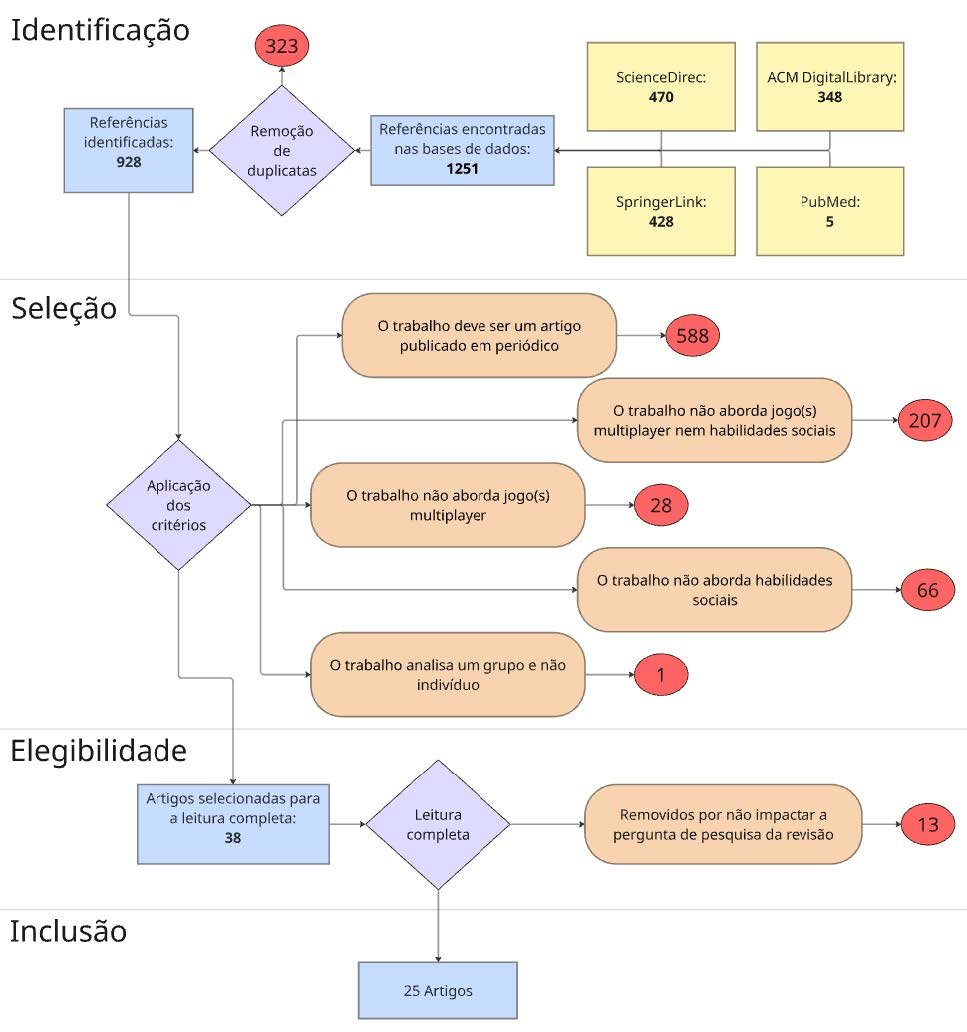
\includegraphics[width=0.8\textwidth]{imgs/fluxograma revisão2.jpeg}
    \caption{Fluxograma do processo de triagem dos estudos}
    \label{fig:fluxo-triagem}
\end{figure}

Por fim, após a leitura de título e resumo, restaram \textbf{38 artigos} que passaram para etapa de leitura completa. A Figura~\ref{fig:fluxo-triagem} ilustra que \textbf{13 artigos} foram removidos por não serem relevantes para o escopo deste trabalho.

\subsection{Conclusão da revisão}

Foi possível chegar a algumas conclusões a partir da revisão sistemática que estão melhor detalhadas no artigo de \cite{Santos2026JogosMultiplayer}, no entanto um dos principais achados foi a predominância dos \textit{Jogos Sérios} como ferramenta de análise e treinamento de habilidades sociais, juntamente com a dificuldade da padronização de métricas para avaliar habilidades sociais, uma vez que esse conjunto de habilidades é muito amplo e na maioria dos trabalhos apenas alguns desses aspectos dessas habilidades são avaliados.

Nesse sentido a revisão sistemática reforçou a necessidade de mais pesquisas que explorem o potencial dos jogos multiplayer como ferramentas de desenvolvimento de habilidades sociais, como o presente trabalho.